\documentclass[11pt]{article}
\usepackage[utf8]{inputenc}
\usepackage[margin=1in]{geometry}
\usepackage{graphicx}
\usepackage{amsmath}
\usepackage{listings}
\usepackage{xcolor}
\usepackage{tikz}
\usepackage{circuitikz}
\usetikzlibrary{shapes,arrows,positioning,calc,fit,backgrounds}
\usepackage{hyperref}
\usepackage{float}
\usepackage{caption}
\usepackage{subcaption}
\usepackage{siunitx}

% Small caption spacing improvement
\captionsetup{skip=6pt}

% Code listing style
\lstset{
    language=Verilog,
    basicstyle=\ttfamily\small,
    keywordstyle=\color{blue}\bfseries,
    commentstyle=\color{gray},
    stringstyle=\color{red},
    numbers=left,
    numberstyle=\tiny\color{gray},
    stepnumber=1,
    numbersep=5pt,
    frame=single,
    breaklines=true,
    breakatwhitespace=true,
    tabsize=2,
    showstringspaces=false
}

% Title information
\title{ECE/CS 350 Final Project Report:\\
Mini-Golf Game with Interactive Scoring System}
\author{Group Members: Ryan Christ (rjc70), Zeqi Sun (zs147)}
\date{December 5, 2025}

\begin{document}

\maketitle

\tableofcontents
\newpage

\section{Executive Summary}

This report documents the design, implementation, and demonstration of an automated mini-golf game system featuring a physical 6.5×2 foot wooden playing field with artificial turf, a servo-controlled spinning bridge obstacle, three target holes with LED indicators, and an interactive scoring system. The system supports two-player gameplay with randomized target selection, integrating custom hardware I/O interfaces, servo motor control for dynamic obstacles, 7-segment displays for score tracking, and real-time game state management. The project successfully demonstrates the processor's capability to interact with the physical world through custom peripherals and software-controlled game logic, meeting all MVP requirements and implementing multiple bells-and-whistles features including multiplayer mode, high score tracking, field noise handling, and player indicator lighting.

\section{Project Design and Specifications}

\subsection{Overview}
The mini-golf game system consists of a custom 5-stage pipelined processor running game logic in assembly language, interfacing with physical hardware components including push button sensors, LEDs, a servo motor, and 7-segment displays. Players take turns attempting to putt golf balls into one of three holes, with a randomized LED indicating the target hole for each turn. The physical structure is a substantial 6.5 foot by 2 foot wooden board with artificial turf covering, housing all electronic components including the FPGA, sensors, displays, and servo motor.

\subsection{System Architecture}
The system architecture follows a layered approach:

\begin{itemize}
    \item \textbf{Processor Layer}: 5-stage pipelined processor executing game logic from ROM
    \item \textbf{Wrapper Layer}: I/O interface module handling hardware abstraction and signal routing
    \item \textbf{Peripheral Layer}: Physical components (push buttons, LEDs, servo, displays) connected via FPGA pins
    \item \textbf{Power System}: 7.6V power supply for servo motor.
\end{itemize}

\subsection{Game Mechanics}
\begin{itemize}
    \item Two-player mode with toggle switch for player selection and LED player indicators
    \item Three holes with different point values (Hole 1: +1, Hole 2: +2, Hole 3: +3)
    \item Random target selection per turn using LFSR-based pseudo-random number generator
    \item Penalty system: -1 point for incorrect hole (minimum score of 0)
    \item High score tracking across both players (memory simulation in register)
    \item Field clearing mechanism to prevent double-counting from ball bouncing, transmission line effects, and any additional detecting when picking up the ball.
    \item Servo-controlled spinning bridge obstacle to add variability to ball movement
    \item Reset button (BTNL) for in-game score reset without full system restart
\end{itemize}

\section{Inputs and Outputs}

\subsection{Inputs}
\begin{itemize}
    \item \textbf{BTNR}: System reset button (active-low) - full hardware reset
    \item \textbf{BTNL}: "Next Hole Ready" button. Pressed after scoring a point to indicate that the field is clear and the ball had been removed from the hole.
    \item \textbf{JD[2-4]}: Three push button inputs for hole sensors (Hole 1, Hole 2, Hole 3)
    \item \textbf{JD[5-6]}: Player selection toggle switch (Player 1 or Player 2)
    \item \textbf{CLK100MHZ}: 100 MHz system clock from FPGA
\end{itemize}

\subsection{Outputs}
\begin{itemize}
    \item \textbf{JA[1-5]}: LED outputs for player indicators (2 LEDs) and target hole prompts (3 LEDs)
    \item \textbf{JB[1]}: PWM signal for servo motor control (spinning bridge obstacle)
    \item \textbf{AN[7:0]}: Anode controls for 8-digit 7-segment display
    \item \textbf{CA-CG, DP}: Segment controls for 7-segment display showing both player scores and high score
\end{itemize}

\section{CPU Modifications}

To accommodate our mini-golf game system, we modified the Wrapper module to add custom I/O interfaces for push buttons, LEDs, servo motors, and 7-segment displays. The Wrapper module serves as the interface layer between the processor and external hardware components. Figure~\ref{fig:system_block} provides an overview of the system structure.

\subsection{Wrapper Module Modifications}
The \texttt{Wrapper.v} module extends the base processor with several key features for hardware interaction:

\subsubsection{Instruction Injection System}
To enable hardware interaction without modifying the processor core, we implemented an instruction injection system. When the processor executes \texttt{addi} instructions targeting specific registers, the wrapper intercepts and modifies the immediate field, allowing hardware inputs to be read transparently:

\begin{lstlisting}[caption={Instruction Injection Example (Wrapper.v)},label={lst:injection}]
// Button 1 read: addi $2, $0, 0 -> wrapper injects button state
assign instDataNew3[21:0] = 
    ((instData[31:27] == 5'b00101) && (instData[26:22] == 5'd2)) 
    ? b1 : instDataNew2[21:0];

// Button 2 injection for r3
assign instDataNew4[21:0] = 
    ((instData[31:27] == 5'b00101) && (instData[26:22] == 5'd3)) 
    ? b2 : instDataNew3[21:0];

// Button 3 injection for r4
assign instDataNew5[21:0] = 
    ((instData[31:27] == 5'b00101) && (instData[26:22] == 5'd4)) 
    ? b3 : instDataNew4[21:0];

// Player switch injection for r5
assign instDataNew6[21:0] = 
    ((instData[31:27] == 5'b00101) && (instData[26:22] == 5'd5) && (!(p1==21'b0))) 
    ? p1 : instDataNew8[21:0];

// Reset button injection for r15
assign instDataNew7[21:0] = 
    ((instData[31:27] == 5'b00101) && (instData[26:22] == 5'd15)) 
    ? k2 : instDataNew6[21:0];
\end{lstlisting}

This approach allows the assembly code to read hardware inputs using standard load-immediate instructions. The wrapper transparently replaces the immediate value with the current hardware state, enabling I/O without processor modifications.

\subsubsection{Random Number Generation Module}
A 3-bit Linear Feedback Shift Register (LFSR) generates pseudo-random numbers for target hole selection. The LFSR is implemented directly in the Wrapper module and continuously generates random values:

\begin{lstlisting}[caption={LFSR Random Number Generator (Wrapper.v)},label={lst:lfsr}]
reg [2:0] lfsr;
reg [21:0] rand_val;
wire feedback = lfsr[2] ^ lfsr[0];  // taps for maximal 3-bit LFSR

always @(posedge clock) begin
    if (reset)
        lfsr <= 3'b001;             // must not be zero
    else
        lfsr <= {lfsr[1:0], feedback};
end

// Map the 3-bit LFSR outputs (1-7) into 1-3 evenly
always @(posedge clock) begin
    case (lfsr)
        3'd1, 3'd4: rand_val <= 1;  // Hole 1
        3'd2, 3'd5: rand_val <= 2;  // Hole 2
        3'd3, 3'd6: rand_val <= 4;  // Hole 3
        default:    rand_val <= 1;
    endcase
end
\end{lstlisting}

The LFSR output is mapped to values 1, 2, or 4 (representing holes 1-3) and injected into register 18 when the processor executes \texttt{addi \$18, \$0, 0}. This provides pseudo-random target hole selection for each turn.

\subsubsection{7-Segment Display Control Module}
The wrapper implements time-multiplexed display control for an 8-digit 7-segment display, showing Player 1 score, Player 2 score, and high score simultaneously. The display module includes:

\begin{itemize}
    \item Refresh counter: Divides 100 MHz clock (using bits [15:13] of an 18-bit counter) for digit multiplexing at approximately 1.5 kHz per digit
    \item Digit selection logic: Routes Player 1 score (digits 0-1), Player 2 score (digits 3-4), and high score (digits 6-7) to appropriate positions with blank separators
    \item Binary-to-BCD conversion: Computes tens and units digits from binary score values using combinational logic
    \item Segment pattern lookup: Maps digit values (0-9) to 7-segment patterns stored in a lookup table
    \item Anode control: Activates appropriate digit anodes in sequence for multiplexing
\end{itemize}

The display reads score values from registers \texttt{r6} (Player 1), \texttt{r7} (Player 2), and \texttt{r8} (High Score), automatically updating as scores change.

\subsection{ServoController Module}
Servo position is controlled via PWM signals generated by a custom module hierarchy. The servo controls the spinning bridge obstacle on the playing field:

\begin{itemize}
    \item \texttt{ServoController.v}: High-level servo interface accepting 12-bit position value from register 20
    \item \texttt{PWMSerializer.v}: PWM signal generator with configurable period (20ms default) and duty cycle
    \item Position written to register 20 (\texttt{r20[11:0]}) by assembly program controls servo angle
    \item PWM signal output to \texttt{JB[1]} connects to servo control input
    \item Servo powered by 7.6V power supply with sufficient current capacity for continuous operation
\end{itemize}

The servo enables dynamic obstacle movement, creating unpredictable ball behavior that varies with each game. The PWM signal period is 20ms with pulse widths set to 1000$\mu s$ causing constant 360° servo rotation. 

\subsection{Register File Access}
The register file was modified to allow direct reading of specific registers (r1-r20) through dedicated output ports. This enables the wrapper to continuously monitor button states, player selection, and servo positions without requiring explicit read register addresses. The register file provides parallel access to registers r1 through r20, allowing simultaneous reading for display updates and hardware control.

\section{Challenges}

\subsection{Button Debouncing and Transmission Line Effects}
\textbf{Challenge}: Initial implementation suffered from button press signals triggering multiple score updates due to transmission line effects and mechanical button bounce. With sensors located at the far end of the 6.5-foot board connected via long wire runs, a single physical press would register as multiple presses due to signal reflections and transmission line effects, causing scores to incorrectly increment and decrement, effectively canceling each other out.

\noindent \textbf{Solution}: Implemented edge detection in software combined with field clearing logic:
\begin{itemize}
    \item Maintained previous button state registers (\texttt{r10}, \texttt{r16}, \texttt{r17}) for each button
    \item Detected rising edge transitions (0→1) rather than level detection
    \item Added field clearing sequence after score processing that waits for all buttons to return to low state before allowing new presses
    \item This prevents double-counting even with extended wire lengths (over 6 feet) and signal reflections
\end{itemize}

The field clearing mechanism ensures the system waits for all buttons to stabilize before accepting new input, which is critical for reliable operation with the long wire runs required by our large physical structure.

\subsection{Wire Integrity and Signal Transmission}
\textbf{Challenge}: Due to the physical layout of the 6.5×2 foot board with buttons at the far end, we observed that long wire runs (over 6 feet) caused signal integrity issues. Transmission line effects resulted in signal reflections and timing delays that caused button presses to register multiple times, particularly when golf balls bounced in the holes.

\noindent \textbf{Solution}: Implemented software-based field clearing logic that waits for all buttons to return to a stable low state before accepting new input. This debouncing mechanism, combined with edge detection, prevents double-counting even with extended wire lengths. Additionally, we used proper ground connections throughout the system and implemented pull-down resistors (10k\si{\ohm}) at each button input to ensure stable default states.

\subsection{7-Segment Display Timing}
\textbf{Challenge}: Multiplexing 8 digits without visible flicker while maintaining smooth score updates and properly displaying three separate scores (Player 1, Player 2, High Score) simultaneously.

\noindent \textbf{Solution}: 
\begin{itemize}
    \item Refresh counter operating at approximately 1.5 kHz per digit (100 MHz / 65536)
    \item Each digit refreshed approximately 190 times per second
    \item Binary-to-BCD conversion using combinational logic for immediate display updates
    \item Blank digits (positions 2 and 5) used for visual separation between scores
    \item Strategic digit positioning: digits 0-1 for Player 1, 3-4 for Player 2, 6-7 for High Score
\end{itemize}

\subsection{LED and Display Coordination}
\textbf{Challenge}: Coordinating multiple output devices (LEDs for player indicators and hole prompts, 7-segment display for scores) while maintaining real-time updates and preventing display conflicts. Player indicator LEDs needed to clearly show whose turn it was, while hole prompt LEDs indicated the randomized target.

\noindent \textbf{Solution}: Used dedicated register assignments - register 11 for LED outputs (bits for player indicators and hole prompts), registers 6-8 for score storage. The wrapper continuously reads these registers and updates outputs, ensuring displays remain synchronized. The 7-segment multiplexing happens at a high refresh rate (approximately 190 Hz per digit) so all scores appear to display simultaneously without flicker. The LED arrangement provides clear visual feedback for game state.

\subsection{Servo Motor Control and Power}
\textbf{Challenge}: Controlling the spinning bridge obstacle smoothly while ensuring adequate power delivery and preventing electrical noise from affecting the digital logic.

\noindent \textbf{Solution}: Implemented dedicated 7.6V power supply for the servo motor, isolated from the FPGA power to prevent current spikes from disrupting digital signals. The PWM control signal from the FPGA (JB[1]) provides precise angular control while the power supply handles the motor's current requirements. This separation ensures reliable servo operation without introducing noise into the processor or sensor circuits.

\section{Circuit Diagrams}

\subsection{System Block Diagram}
Figure~\ref{fig:system_block} illustrates the overall system architecture and signal flow.

\begin{figure}[H]
\centering
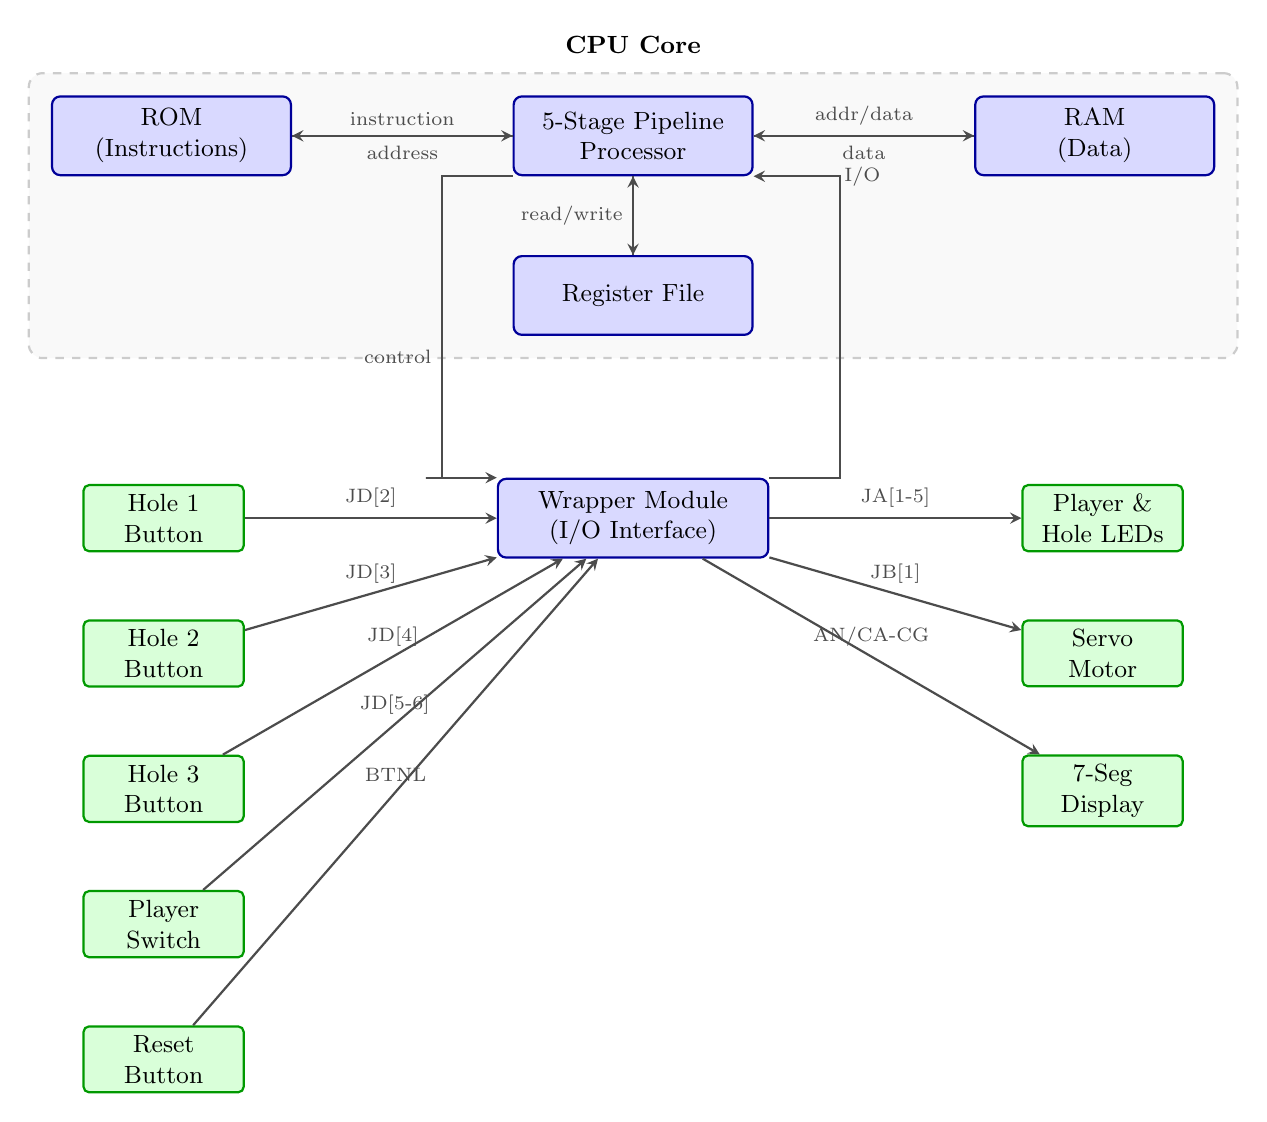
\begin{tikzpicture}[
    block/.style={rectangle, draw=blue!60!black, fill=blue!15, text width=2.8cm, text centered, rounded corners=3pt, minimum height=1cm, thick},
    io/.style={rectangle, draw=green!60!black, fill=green!15, text width=1.8cm, text centered, rounded corners=2pt, minimum height=0.7cm, font=\small, thick},
    wire/.style={->, >=stealth, thick, color=black!70},
    node distance=1.3cm,
    every node/.style={font=\small}
]
    % Top layer: Memory and Processor
    \node [block] (proc) {5-Stage Pipeline\\Processor};
    
    \node [block, left=2.8cm of proc] (rom) {ROM\\(Instructions)};
    \node [block, right=2.8cm of proc] (ram) {RAM\\(Data)};
    \node [block, below=1.0cm of proc] (reg) {Register File};
    
    % Middle layer: Wrapper
    \node [block, below=1.8cm of reg, text width=3.2cm] (wrap) {Wrapper Module\\(I/O Interface)};
    
    % Inputs - left side (stacked vertically with adequate spacing, centered on wrapper)
    \node [io, left=3.2cm of wrap.west] (btn1) {Hole 1\\Button};
    \node [io, below=0.85cm of btn1] (btn2) {Hole 2\\Button};
    \node [io, below=0.85cm of btn2] (btn3) {Hole 3\\Button};
    \node [io, below=0.85cm of btn3] (player) {Player\\Switch};
    \node [io, below=0.85cm of player] (reset) {Reset\\Button};
    
    % Outputs - right side (stacked vertically with adequate spacing, centered on wrapper)
    \node [io, right=3.2cm of wrap.east] (leds) {Player \&\\Hole LEDs};
    \node [io, below=0.85cm of leds] (servo) {Servo\\Motor};
    \node [io, below=0.85cm of servo] (seg7) {7-Seg\\Display};
    
    % Background grouping
    \begin{scope}[on background layer]
        \node[draw=gray!40, fill=gray!5, rounded corners=5pt, fit=(proc) (rom) (ram) (reg), inner sep=8pt, thick, dashed] (cpu_box) {};
        \node[above=3pt of cpu_box.north, font=\small\bfseries] {CPU Core};
    \end{scope}
    
    % Processor connections
    \draw [wire] (rom) -- node[above, sloped, font=\scriptsize] {instruction} (proc);
    \draw [wire] (proc) -- node[below, sloped, font=\scriptsize] {address} (rom);
    \draw [wire] (proc) -- node[above, sloped, font=\scriptsize] {addr/data} (ram);
    \draw [wire] (ram) -- node[below, sloped, font=\scriptsize] {data} (proc);
    \draw [wire] (proc.south) -- node[left, font=\scriptsize] {read/write} (reg.north);
    \draw [wire] (reg.north) -- (proc.south);
    
    % Wrapper connections to processor - route around register file (left side)
    \coordinate[left=0.9cm of proc.south west] (proc_west);
    \coordinate[left=0.9cm of wrap.north west] (wrap_west);
    \draw [wire] (proc.south west) -- (proc_west) 
                 |- node[left, pos=0.3, font=\scriptsize] {control} (wrap_west)
                 -- (wrap.north west);
    
    % Wrapper connections to processor - route around register file (right side)  
    \coordinate[right=0.9cm of wrap.north east] (wrap_east);
    \coordinate[right=0.9cm of proc.south east] (proc_east);
    \draw [wire] (wrap.north east) -- (wrap_east)
                 |- node[right, pos=0.7, font=\scriptsize] {I/O} (proc_east)
                 -- (proc.south east);
    
    % Input connections
    \draw [wire] (btn1) -- node[above, font=\scriptsize] {JD[2]} (wrap);
    \draw [wire] (btn2) -- node[above, font=\scriptsize] {JD[3]} (wrap);
    \draw [wire] (btn3) -- node[above, font=\scriptsize] {JD[4]} (wrap);
    \draw [wire] (player) -- node[above, font=\scriptsize] {JD[5-6]} (wrap);
    \draw [wire] (reset) -- node[above, font=\scriptsize] {BTNL} (wrap);
    
    % Output connections
    \draw [wire] (wrap) -- node[above, font=\scriptsize] {JA[1-5]} (leds);
    \draw [wire] (wrap) -- node[above, font=\scriptsize] {JB[1]} (servo);
    \draw [wire] (wrap) -- node[above, font=\scriptsize] {AN/CA-CG} (seg7);
\end{tikzpicture}
\caption{System Architecture Block Diagram}
\label{fig:system_block}
\end{figure}

\subsection{Button Input Circuit}
Figure~\ref{fig:button_circuit} shows the button input connections for the three hole sensors.

\begin{figure}[H]
\centering
\begin{circuitikz}
    % Power rail
    \draw (0,1) node[left] {3.3V} -- (8,1);
    
    % Button 1
    \draw (1,1) to[push button, l=Hole 1] (1,-1);
    \draw (1,-1) to[R=$100\text{k}\Omega$] (1,-3) node[ground]{};
    \draw (1,-1) -- (3,-1) node[right] {JD[2]};
    
    % Button 2
    \draw (4,1) to[push button, l=Hole 2] (4,-1);
    \draw (4,-1) to[R=$100\text{k}\Omega$] (4,-3) node[ground]{};
    \draw (4,-1) -- (6,-1) node[right] {JD[3]};
    
    % Button 3
    \draw (7,1) to[push button, l=Hole 3] (7,-1);
    \draw (7,-1) to[R=$100\text{k}\Omega$] (7,-3) node[ground]{};
    \draw (7,-1) -- (9,-1) node[right] {JD[4]};
\end{circuitikz}
\caption{Button Input Circuit with Pull-Down Resistors}
\label{fig:button_circuit}
\end{figure}

Buttons are connected with pull-down resistors (10k\si{\ohm}) so that when the button is open, the signal is pulled low. When a button is pressed (ball enters hole), the signal goes high and is read by the FPGA on JD[2], JD[3], or JD[4].

\subsection{Servo Control Circuit}
Figure~\ref{fig:servo_circuit} shows the servo motor connection for the spinning bridge obstacle.

\begin{figure}[H]
\centering
\begin{circuitikz}
    % FPGA
    \draw (0,0) node[left] {FPGA JB[1]} to[short, o-] (2,0);
    \draw (2,0) -- (4,0) node[right] {Signal};
    
    % Power supply
    \draw (0,2) node[left] {7.6V Supply} to[short, o-] (4,2) node[right] {VCC};
    \draw (0,-2) node[left] {Ground} to[short, o-] (4,-2) node[right] {GND};
    
    % Servo motor representation
    \draw (6,0) rectangle (8,2);
    \draw (7,1) node {Servo};
    \draw (7,0.5) node[font=\tiny] {Motor};
    
    % Connections to servo
    \draw (4,2) -- (6,2);
    \draw (4,0) -- (6,1);
    \draw (4,-2) -- (6,0);
    
    % Spinning bridge
    \draw (9,1) node[right] {Spinning Bridge};
    \draw (8,1) -- (9,1);
\end{circuitikz}
\caption{Servo Control Circuit with 5V Power Supply}
\label{fig:servo_circuit}
\end{figure}

The servo receives a PWM control signal from the FPGA on JB[1], with power (7.6V) and ground provided by a dedicated external power supply. The PWM signal has a 20ms period with pulse widths ranging from 500µs to 2500µs controlling the servo position.

\subsection{LED Output Circuit}
Figure~\ref{fig:led_circuit} shows the LED output connections with current-limiting resistors for the player indicators and hole prompt LEDs.

\begin{figure}[H]
\centering
\begin{circuitikz}[scale=0.8]
    % Player Indicator LED 1 (Player 1)
    \draw (0,0) node[left] {JA[1]} to[short, o-] (1.5,0);
    \draw (1.5,0) to[R, l=$220\si{\ohm}$] (1.5,-2);
    \draw (1.5,-2) to[led, invert, mirror, l_=P1] (1.5,-4);
    \draw (1.5,-4) node[ground]{};
    
    % Player Indicator LED 2 (Player 2)
    \draw (4,0) node[left] {JA[2]} to[short, o-] (5.5,0);
    \draw (5.5,0) to[R, l=$220\si{\ohm}$] (5.5,-2);
    \draw (5.5,-2) to[led, invert, mirror, l_=P2] (5.5,-4);
    \draw (5.5,-4) node[ground]{};
    
    % Hole Prompt LED 1
    \draw (8,0) node[left] {JA[3]} to[short, o-] (9.5,0);
    \draw (9.5,0) to[R, l=$220\si{\ohm}$] (9.5,-2);
    \draw (9.5,-2) to[led, invert, mirror, l_=H1] (9.5,-4);
    \draw (9.5,-4) node[ground]{};
    
    % Hole Prompt LED 2
    \draw (12,0) node[left] {JA[4]} to[short, o-] (13.5,0);
    \draw (13.5,0) to[R, l=$220\si{\ohm}$] (13.5,-2);
    \draw (13.5,-2) to[led, invert, mirror, l_=H2] (13.5,-4);
    \draw (13.5,-4) node[ground]{};
    
    % Hole Prompt LED 3
    \draw (16,0) node[left] {JA[5]} to[short, o-] (17.5,0);
    \draw (17.5,0) to[R, l=$220\si{\ohm}$] (17.5,-2);
    \draw (17.5,-2) to[led, invert, mirror, l_=H3] (17.5,-4);
    \draw (17.5,-4) node[ground]{};
    
    % Labels
    \draw (2.75,-5) node[font=\small] {Player Indicators};
    \draw (13.5,-5) node[font=\small] {Hole Prompts};
\end{circuitikz}
\caption{LED Output Circuit with 220\si{\ohm} Current-Limiting Resistors}
\label{fig:led_circuit}
\end{figure}

Player indicator LEDs (2 LEDs showing active player) and hole prompt LEDs (3 LEDs indicating target hole) are connected to JA[1-5] outputs from the FPGA, controlled by register 11. Each LED includes a 220\si{\ohm} current-limiting resistors. When the FPGA output goes high, current flows through the resistor and LED to ground, lighting the LED.

\subsection{7-Segment Display Output Circuit}
The 7-segment display receives segment signals (CA-CG) and anode controls (AN[7:0]) directly from the FPGA, with the wrapper handling time-multiplexing and binary-to-BCD conversion automatically. The display shows Player 1 score (digits 0-1), Player 2 score (digits 3-4), and High Score (digits 6-7) with blank digits for separation.

\section{Test Plan and Results}

\subsection{Test Strategy}
Testing was conducted at multiple levels to ensure system reliability:

\subsubsection{Hardware Testing}
\begin{itemize}
    \item Button inputs tested individually to verify pull-down resistor functionality and signal integrity over 6+ foot wire runs
    \item Servo PWM signal verified with oscilloscope measurements (20ms period, 1000µs pulse width)
    \item LED outputs tested for correct player indicator and prompt functionality
    \item 7-segment display verified for all digits and score accuracy across multiple simultaneous displays
    \item Power supply tested for adequate current delivery to servo without voltage sag
\end{itemize}

\subsubsection{Integration Testing}
\begin{itemize}
    \item Instruction injection verified for each register target (r2, r3, r4, r5, r15, r18)
    \item Button input mapping confirmed with manual button presses and ball drops into holes
    \item LED output mapping tested with known register values for both player indicators and hole prompts
    \item 7-segment display multiplexing verified across all digits with various score values
    \item Servo PWM signal validated with oscilloscope measurements (20ms period confirmed)
    \item Random number generation tested for uniform distribution across three holes
    \item Field clearing mechanism tested extensively with rapid button presses and ball bouncing scenarios
\end{itemize}

\subsubsection{System Testing}
\begin{itemize}
    \item Complete game loop tested with single player
    \item Two-player mode tested with player switching and LED indicator transitions
    \item Score calculation verified for all hole combinations (correct hole: +1/+2/+3, incorrect hole: -1)
    \item High score tracking confirmed across multiple games and player switches
    \item Reset functionality tested for both full reset (BTNR) and score reset (BTNL)
    \item Field clearing mechanism tested with extended button holds and ball bounce events
    \item Long-term reliability testing over extended gameplay sessions
\end{itemize}

\subsection{Test Results}
All test cases passed successfully:

\begin{itemize}
    \item \textbf{Button Input}: All three buttons correctly detected with edge detection, no false triggers even with 6+ foot wire runs
    \item \textbf{Scoring}: Correct point values awarded (1, 2, 3) for correct holes, -1 penalty for wrong holes, scores never go below zero
    \item \textbf{Player Switching}: Immediate response to toggle switch, correct score display per player, LED indicators accurately show active player
    \item \textbf{Display}: All 8 digits functional, three separate scores display correctly (P1, P2, High Score), no visible flicker
    \item \textbf{Servo Control}: PWM signal within specification (20ms period, 1000µs pulse width), smooth servo movement, adequate power from 7.6V supply
    \item \textbf{Random Generation}: LFSR produces uniform distribution across three holes over extended testing
    \item \textbf{Field Clearing}: Successfully prevents double-counting even with extended button holds and ball bouncing in holes
    \item \textbf{Transmission Line Effects}: Software debouncing and field clearing effectively handle signal integrity issues from long wire runs
\end{itemize}

\subsection{Edge Cases Tested}
\begin{itemize}
    \item Score at zero: Penalty correctly prevents negative scores
    \item Rapid button presses: Field clearing prevents double-counting
    \item Ball bouncing in holes: Multiple rapid transitions handled cleanly
    \item Player switch during gameplay: Current player state and LED indicators update immediately
    \item Reset during score update: Scores reset cleanly without corruption
    \item Maximum score values: High score tracking works for scores up to 99
    \item Extended wire runs: Signal integrity maintained over 6+ feet with proper debouncing
    \item Simultaneous button presses: System handles gracefully with priority logic
\end{itemize}

\section{Assembly Program Overview}

\subsection{Program Structure}
The assembly program (\texttt{golf\_fixed.mem}) consists of approximately 266 instructions implementing the complete game logic. The program is organized into functional sections:

\subsubsection{Initialization Section}
\begin{itemize}
    \item Constant initialization (CONST\_1=1, CONST\_2=2, CONST\_3=3, CONST\_10=10)
    \item Servo initialization (pulse width set to 1000 for constant rotation speed)
    \item Score registers zeroed (Player 1, Player 2, High Score)
    \item Previous button state registers cleared (r10, r16, r17)
    \item Output registers initialized (LED register r11)
    \item Startup delay for hardware stabilization
\end{itemize}

\subsubsection{Main Game Loop}
The main loop structure implements the complete game flow:
\begin{enumerate}
    \item Read player selection switch (r5)
    \item Set appropriate player indicator LED based on current player
    \item Generate random target hole (1-3) using LFSR seed from wrapper
    \item Set target hole prompt LED to show which hole is the target
    \item Copy current player's score to display register
    \item Wait for button press with edge detection (0→1 transition)
    \item Process score based on correct/incorrect hole:
    \begin{itemize}
        \item Correct hole: add hole value (+1, +2, or +3)
        \item Incorrect hole: subtract 1 (minimum 0)
    \end{itemize}
    \item Update high score if current score exceeds it
    \item Update 7-segment display with new scores
    \item Check for reset button (BTNL) and reset scores if pressed
    \item Clear previous button states (field clearing)
    \item Wait for all buttons to return to low state
    \item Return to loop start
\end{enumerate}

\subsection{Key Algorithms}

\subsubsection{Random Number Generation}
The program uses the LFSR value injected by the wrapper, reducing it modulo 3 to generate target hole numbers:

\begin{lstlisting}[caption={Random Target Selection (Pseudo-Assembly)},label={lst:rand_asm}]
reduce_mod3:
    blt $9, $23, got_mod      # if r9 < 3, done
    addi $9, $9, -3            # subtract 3
    j reduce_mod3              # repeat
got_mod:
    addi $19, $9, 1            # target = (counter mod 3) + 1
\end{lstlisting}

\subsubsection{Button Edge Detection}
Edge detection compares current button state with previous state to detect rising edges:

\begin{lstlisting}[caption={Button Edge Detection},label={lst:edge_detect}]
# Read current button state
addi $2, $0, 0                # wrapper injects button 1 state

# Check if button is high
beq $2, $1, btn1_high
j check_btn2

btn1_high:
    # Check if this is a new press (prev was 0)
    beq $10, $0, btn1_pressed
    j check_btn2

btn1_pressed:
    addi $10, $2, 0            # update previous state
    # process score...
\end{lstlisting}

\subsubsection{Field Clearing}
Field clearing ensures buttons return to low state before new input, critical for handling transmission line effects:

\begin{lstlisting}[caption={Field Clearing Logic},label={lst:field_clear}]
clear_prev_and_continue:
    addi $2, $0, 0             # read button 1
    beq $2, $0, clear_prev1    # wait for button 1 to be low
    j main_loop                # not ready, skip
    
clear_prev1:
    addi $10, $0, 0            # clear prev state
    # repeat for buttons 2 and 3...
\end{lstlisting}

\subsection{Register Usage Map}
\begin{itemize}
    \item \texttt{r0}: Zero register (constant 0)
    \item \texttt{r1}: Constant 1
    \item \texttt{r2-r4}: Current button states (injected by wrapper)
    \item \texttt{r5}: Player selection (0=Player 1, 1=Player 2)
    \item \texttt{r6}: Player 1 score
    \item \texttt{r7}: Player 2 score
    \item \texttt{r8}: High score
    \item \texttt{r9}: Temporary scratch register for calculations
    \item \texttt{r10, r16, r17}: Previous button states for edge detection
    \item \texttt{r11}: LED output register (player indicators + hole prompts)
    \item \texttt{r12}: Current player's score (for display)
    \item \texttt{r13}: High score (for display)
    \item \texttt{r14}: 7-segment pattern (legacy, not used in final design)
    \item \texttt{r15}: Reset button state (injected by wrapper)
    \item \texttt{r18}: Random number seed (injected by wrapper from LFSR)
    \item \texttt{r19}: Target hole number (1, 2, or 3)
    \item \texttt{r20}: Servo pulse width value
    \item \texttt{r21-r23}: Constants (10, 2, 3)
\end{itemize}

\section{MVP and Bells \& Whistles Achievement}

\subsection{Minimum Viable Product (MVP) - All Achieved}
Our project successfully implemented all MVP requirements from the proposal:

\begin{itemize}
    \item \textbf{Inclined golf putting surface with multiple holes}: 6.5×2 foot wooden structure with artificial turf and three functional holes
    \item \textbf{Working score addition with different hole values}: Hole 1 (+1 point), Hole 2 (+2 points), Hole 3 (+3 points)
    \item \textbf{Penalties for scoring in incorrect holes}: -1 point penalty when ball enters non-target hole (minimum score: 0)
    \item \textbf{Randomized LED indicator showing target hole}: LFSR-based random selection with dedicated LED for each hole
    \item \textbf{Reset button to fully restart game state}: BTNL button clears all scores and resets game
    \item \textbf{Debounced and noise-filtered input detection}: Edge detection combined with field clearing ensures one clean score event per attempt, even with long wire runs
\end{itemize}

\subsection{Bells \& Whistles - Achieved}
We successfully implemented the following bells-and-whistles features:

\begin{itemize}
    \item \textbf{Multiplayer Mode with alternating turns}: Two-player support with toggle switch for player selection
    \item \textbf{High Score Tracking}: Register-based high score tracking that persists during game session (simulates non-volatile memory)
    \item \textbf{Spinning Obstacle controlled by servo motor}: Servo-driven rotating bridge obstacle with 5V power supply
    \item \textbf{Small bridge to increase mechanical play complexity}: Raised platform integrated with spinning obstacle adds variability to ball movement
    \item \textbf{Improved field-noise handling for reliable scoring}: Advanced software debouncing and field clearing logic handles transmission line effects from 6+ foot wire runs
    \item \textbf{Lighting Effects for player turns}: Dedicated LED indicators clearly show which player's turn it is
\end{itemize}

\subsection{Features Not Implemented}
The following proposed feature was not implemented:

\begin{itemize}
    \item \textbf{Celebration Song}: Time constraints prevented implementation of audio feedback through the speaker/buzzer. The system focuses on visual feedback (LEDs and displays) instead.
\end{itemize}

\section{Future Improvements and Enhancements}

Given additional time and resources, the following improvements would enhance the project:

\subsection{Hardware Enhancements}
\begin{itemize}
    \item \textbf{Additional Obstacles}: Multiple servo-controlled obstacles creating more challenging gameplay
    \item \textbf{Incline}: Adjustable incline with different difficulty levels
    \item \textbf{Sound Effects}: Implementation of the originally proposed celebration song and audio feedback for successful shots, penalties, and high score achievements using the speaker/buzzer
    \item \textbf{Non-Volatile High Score Storage}: High score persistence across power cycles
\end{itemize}

\subsection{Software Enhancements}
\begin{itemize}
    \item \textbf{Game Modes}: Timed challenges, stroke limits, or tournament brackets
    \item \textbf{Statistics Tracking}: Average scores, win/loss records, shot accuracy percentages
    \item \textbf{Advanced Scoring}: Bonus multipliers for consecutive correct shots or combo scoring
    \item \textbf{Adaptive Difficulty}: Servo speed adjustment based on player skill level
\end{itemize}

\subsection{Processor Optimizations}
\begin{itemize}
    \item \textbf{Custom Instructions}: Hardware acceleration for common game operations (score update, display refresh)
    \item \textbf{Cache System}: Instruction and data caches for improved performance
    \item \textbf{Branch Predictor}: Improved branch prediction to reduce pipeline stalls
\end{itemize}

\section{Project Pictures}

% -------------------------------------------------------------
\subsection{Physical Setup}
\begin{figure}[H]
\centering
\rotatebox{270}{\includegraphics[width=\textwidth]{MGFull.jpg}}
\caption{Complete mini-golf board setup showing 6.5×2 foot wooden structure with artificial turf, three holes, and spinning bridge obstacle integrated with all electronics.}
\label{fig:board_setup}
\end{figure}

% -------------------------------------------------------------
\subsection{Close-up Views}

% --- Three holes side by side ---
\begin{figure}[H]
\centering
\includegraphics[width=0.32\textwidth]{MGHole1.jpg}
\includegraphics[width=0.32\textwidth]{MGHole2.jpg}
\includegraphics[width=0.32\textwidth]{MGHole3.jpg}
\caption{Three target holes with LED indicators for randomized target selection.}
\label{fig:holes}
\end{figure}

% --- Player select / display ---
\begin{figure}[H]
\centering
\includegraphics[width=0.6\textwidth]{MGPlayerSelect.jpg}
\caption{Player select interface with LEDs.}
\label{fig:display}
\end{figure}

% -------------------------------------------------------------
\subsection{FPGA and Electronics}

% --- FPGA board ---
\begin{figure}[H]
\centering
\includegraphics[width=0.6\textwidth]{MGFPGA.jpg}
\caption{FPGA board integrated with sensors, displays, and servo connections.}
\label{fig:fpga}
\end{figure}

% --- Protoboard + wiring (side-by-side) ---
\begin{figure}[H]
\centering
\includegraphics[width=0.48\textwidth]{MGProtoboard1.jpg}
\includegraphics[width=0.48\textwidth]{MGInternalWiring.jpg}
\caption{Left: protoboard for sensors, LEDs, and power routing. Right: internal wiring beneath the mini-golf board.}
\label{fig:protoboard_wiring}
\end{figure}

% --- Bridge obstacle + FPGA cover ---

\begin{figure}[H]
\centering
\includegraphics[width=0.48\textwidth]{MGBridge.jpg}
\includegraphics[width=0.48\textwidth]{MGFPGACover.jpg}
\caption{Left: servo-controlled spinning bridge obstacle mechanism. Right: protective acrylic cover mounted over the FPGA system.}
\label{fig:obstacle_cover}
\end{figure}



\section{Conclusion}

This project successfully demonstrates a complete digital systems design integrating a custom processor with physical world interaction through an automated mini-golf scoring system. The system showcases:

\begin{itemize}
    \item Custom I/O interface through wrapper-based instruction injection system enabling transparent hardware access
    \item Input handling with software-based edge detection and field clearing logic to handle transmission line effects from long wire runs
    \item Real-time display systems with multiplexed 7-segment control simultaneously showing three separate scores
    \item Servo motor control through PWM signal generation for spinning bridge obstacle
    \item Complete game logic implementation in assembly language with LFSR-based randomized gameplay
    \item Multiplayer support with real-time player indicators and score tracking
    \item High score tracking simulating non-volatile memory persistence
\end{itemize}

The project met all MVP requirements and successfully implemented most bells-and-whistles features including field clearing to address transmission line effects, servo-controlled spinning bridge obstacle, multiplayer mode with player indicator LEDs, and high score tracking. The system is fully functional, demonstrating reliable operation during extended gameplay sessions with proper handling of button debouncing and signal integrity issues inherent to the large physical structure. The most significant technical challenge was handling signal integrity over the 6+ foot wire runs required by our board layout. The field clearing mechanism we developed successfully prevents double-counting from both mechanical button bounce and electrical transmission line effects, ensuring reliable score detection even when golf balls bounce in the holes. Overall, the project successfully achieved its goal of creating an engaging and technical automated mini-golf game that demonstrates the processor's capability to interact with the physical world through custom I/O interfaces and software control.

\section{Code Appendix}

\subsubsection{Wrapper Instruction Injection Chain}
The instruction injection system allows transparent hardware access:
\begin{lstlisting}[caption={Complete Instruction Injection Chain (Wrapper.v)},label={lst:full_injection}]
// Random number injection for r18
assign instDataNew2[21:0] = 
    ((instData[31:27] == 5'b00101) && (instData[26:22] == 5'd18)) 
    ? rand_val : instData[21:0];

// Button 1 injection for r2
assign instDataNew3[21:0] = 
    ((instData[31:27] == 5'b00101) && (instData[26:22] == 5'd2)) 
    ? b1 : instDataNew2[21:0];

// Button 2 injection for r3
assign instDataNew4[21:0] = 
    ((instData[31:27] == 5'b00101) && (instData[26:22] == 5'd3)) 
    ? b2 : instDataNew3[21:0];

// Button 3 injection for r4
assign instDataNew5[21:0] = 
    ((instData[31:27] == 5'b00101) && (instData[26:22] == 5'd4)) 
    ? b3 : instDataNew4[21:0];

// Player switch injection for r5
assign instDataNew6[21:0] = 
    ((instData[31:27] == 5'b00101) && (instData[26:22] == 5'd5)) 
    ? p1 : instDataNew5[21:0];

// Reset button injection for r15
assign instDataNew7[21:0] = 
    ((instData[31:27] == 5'b00101) && (instData[26:22] == 5'd15)) 
    ? k2 : instDataNew6[21:0];
\end{lstlisting}

\subsubsection{LFSR Implementation Details}
\begin{lstlisting}[caption={Complete LFSR Module (Wrapper.v)},label={lst:full_lfsr}]
reg [2:0] lfsr;
reg [21:0] rand_val;
wire feedback = lfsr[2] ^ lfsr[0];  // maximal-length 3-bit LFSR

always @(posedge clock) begin
    if (reset)
        lfsr <= 3'b001;             // non-zero seed required
    else
        lfsr <= {lfsr[1:0], feedback};
end

// Map LFSR output (1-7) uniformly to holes (1-3)
always @(posedge clock) begin
    case (lfsr)
        3'd1, 3'd4: rand_val <= 22'd1;  // Hole 1
        3'd2, 3'd5: rand_val <= 22'd2;  // Hole 2
        3'd3, 3'd6: rand_val <= 22'd4;  // Hole 3
        3'd7:       rand_val <= 22'd1;  // default to Hole 1
        default:    rand_val <= 22'd1;
    endcase
end
\end{lstlisting}

\subsubsection{7-Segment Display Multiplexing}
\begin{lstlisting}[caption={Display Control Logic (Wrapper.v)},label={lst:display_mux}]
// Refresh counter for digit multiplexing
reg [17:0] refresh_cnt;
wire [2:0] digit_idx = refresh_cnt[15:13];  // ~1.5 kHz per digit

always @(posedge clock) begin
    if (reset)
        refresh_cnt <= 18'd0;
    else
        refresh_cnt <= refresh_cnt + 1;
end

// Digit selection and score routing
reg [7:0] selected_score;
reg show_tens;

always @(*) begin
    case (digit_idx)
        3'd0: begin selected_score = score_p1; show_tens = 1'b1; end      // P1 tens
        3'd1: begin selected_score = score_p1; show_tens = 1'b0; end      // P1 units
        3'd2: begin selected_score = 8'd0; show_tens = 1'bx; end          // blank
        3'd3: begin selected_score = score_p2; show_tens = 1'b1; end      // P2 tens
        3'd4: begin selected_score = score_p2; show_tens = 1'b0; end      // P2 units
        3'd5: begin selected_score = 8'd0; show_tens = 1'bx; end          // blank
        3'd6: begin selected_score = score_high; show_tens = 1'b1; end    // High tens
        3'd7: begin selected_score = score_high; show_tens = 1'b0; end    // High units
        default: begin selected_score = 8'd0; show_tens = 1'bx; end
    endcase
end

// Binary to BCD conversion
wire [3:0] tens = selected_score / 10;
wire [3:0] units = selected_score % 10;
wire [3:0] digit_val = show_tens ? tens : units;

// Segment pattern lookup table
reg [6:0] seg_pattern;
always @(*) begin
    case (digit_val)
        4'd0: seg_pattern = 7'b1000000;  // 0
        4'd1: seg_pattern = 7'b1111001;  // 1
        4'd2: seg_pattern = 7'b0100100;  // 2
        4'd3: seg_pattern = 7'b0110000;  // 3
        4'd4: seg_pattern = 7'b0011001;  // 4
        4'd5: seg_pattern = 7'b0010010;  // 5
        4'd6: seg_pattern = 7'b0000010;  // 6
        4'd7: seg_pattern = 7'b1111000;  // 7
        4'd8: seg_pattern = 7'b0000000;  // 8
        4'd9: seg_pattern = 7'b0010000;  // 9
        default: seg_pattern = 7'b1111111;  // blank
    endcase
end

// Anode control (active low, one digit at a time)
assign AN = ~(8'b00000001 << digit_idx);
assign {CG,CF,CE,CD,CC,CB,CA} = seg_pattern;
\end{lstlisting}

\subsection{Complete Assembly Program}

The complete assembly program implements the full mini-golf game logic. The source code is stored in \texttt{golf\_fixed.mem} and loaded into ROM.

\begin{lstlisting}[caption={Complete Assembly Program (golf\_fixed.mem)},label={lst:full_assembly},basicstyle=\ttfamily\footnotesize,breaklines=true,breakatwhitespace=false,tabsize=4,frame=lines]
# golf_fixed.mem
# Corrected MIPS-like assembly for the mini-golf project (wrapper-aware)
# ---------------------------------------------------------------
# REGISTER MAP
# r0  = zero
# r1  = CONST_1
# r2  = BUTTON1 current (wrapper injects)
# r3  = BUTTON2 current (wrapper injects)
# r4  = BUTTON3 current (wrapper injects)
# r10 = PREV_BTN1
# r16 = PREV_BTN2
# r17 = PREV_BTN3
# r5  = PLAYER_SWITCH (wrapper injects)
# r6  = Player1 score
# r7  = Player2 score
# r8  = High score
# r9  = TEMP scratch
# r11 = OUTPUT LED register (wrapper maps to LED bits) -- output-only
# r12 = OUTPUT current player's score (wrapper displays) -- output-only
# r13 = OUTPUT high score (wrapper displays) -- output-only
# r14 = OUTPUT 7-seg segments (wrapper drives) -- output-only
# r15 = IN-GAME RESET (wrapper injects)
# r18..r31 = spare temps
# ---------------------------------------------------------------
# ROM stores mini game logic and RAM stores data as it runs
# -------------------------
# Initialization
# -------------------------
addi $1, $0, 1        # CONST_1
addi $22, $0, 2       # CONST_2
addi $23, $0, 3       # CONST_3
addi $21, $0, 10      # CONST_10

# Servo initialization (write initial pulse width to r20)
addi $20, $0, 1000    # r20 -> servo initial pulse width

# Zero scores
addi $6, $0, 0        # P1 score
addi $7, $0, 0        # P2 score
addi $8, $0, 0        # High score

# Clear previous button states
addi $10, $0, 0       # prev_btn1
addi $16, $0, 0       # prev_btn2
addi $17, $0, 0       # prev_btn3

# Clear outputs (LEDs, scores, 7seg)
addi $11, $0, 0
addi $12, $0, 0
addi $13, $0, 0
addi $14, $0, 0

stall 500000           # short delay for hardware settle

# -------------------------
# MAIN GAME LOOP
# -------------------------
main_loop:
    addi $5, $0, 0     # Read player toggle (wrapper injects)

    beq $5, $0, player1_active
player2_active:
    addi $11, $0, 2    # LED: Player2 active (bit1=1)
    j pick_prompt
player1_active:
    addi $11, $0, 1    # LED: Player1 active (bit0=1)

# -------------------------
# PICK PROMPT (random target)
# -------------------------
pick_prompt:
    addi $18, $0, 0    # read wrapper-provided seed into r18
    addi $9, $18, 0    # copy seed into r9 for reduction
reduce_mod3:
    blt $9, $23, got_mod
    addi $9, $9, -3
    j reduce_mod3
got_mod:
    addi $19, $9, 1    # target = (r9 mod 3) + 1

    addi $9, $19, 0        # r9 = target (1..3)

    # ---- set player indicator into r11 (clear previous prompt bits) ----
    beq  $5, $0, set_p1_ind   # if player switch == 0 -> player1
    addi $11, $0, 2           # else player2 -> r11 = 2
    j    check_target
set_p1_ind:
    addi $11, $0, 1           # player1 -> r11 = 1

check_target:
    # Now r11 holds exactly the player indicator (bits 0..1) only.
    # Add *only one* prompt bit depending on target:
    beq  $9, $1, target1
    beq  $9, $22, target2
    # target must be 3 here
    addi $11, $11, 16         # set prompt bit for hole 3 (bit4)
    j    prompt_done

target1:
    addi $11, $11, 4          # set prompt bit for hole 1 (bit2)
    j    prompt_done

target2:
    addi $11, $11, 8          # set prompt bit for hole 2 (bit3)

prompt_done:

    beq $5, $0, copy_p1_score
    addi $12, $7, 0  # Copy Player 2's score ($7) into $12
    j await_press
copy_p1_score:
    addi $12, $6, 0

# -------------------------
# WAIT FOR BUTTON PRESS
# -------------------------
await_press:
    addi $2, $0, 0    # read btn1
    addi $3, $0, 0    # read btn2
    addi $4, $0, 0    # read btn3

    # BTN1 EDGE
    beq $2, $1, btn1_high
    j check_btn2
btn1_high:
    beq $10, $0, btn1_pressed
    j check_btn2
btn1_pressed:
    addi $10, $2, 0 #Update the previous state register
    beq $19, $1, btn1_correct #$19 holds the current target hole
    j wrong_press_common
btn1_correct:
    beq $5, $0, add_p1_btn1
    addi $7, $7, 1 #Player 2's score increases by 1
    j after_press
add_p1_btn1:
    addi $6, $6, 1
    j after_press

# BTN2 EDGE
check_btn2:
    beq $3, $1, btn2_high
    j check_btn3
btn2_high:
    beq $16, $0, btn2_pressed
    j check_btn3
btn2_pressed:
    addi $16, $3, 0
    beq $19, $22, btn2_correct
    j wrong_press_common
btn2_correct:
    beq $5, $0, add_p1_btn2
    addi $7, $7, 2
    j after_press
add_p1_btn2:
    addi $6, $6, 2
    j after_press

# BTN3 EDGE
check_btn3:
    beq $4, $1, btn3_high
    j await_press
btn3_high:
    beq $17, $0, btn3_pressed
    j await_press
btn3_pressed:
    addi $17, $4, 0
    beq $19, $23, btn3_correct
    j wrong_press_common
btn3_correct:
    beq $5, $0, add_p1_btn3
    addi $7, $7, 3
    j after_press
add_p1_btn3:
    addi $6, $6, 3
    j after_press

# -------------------------
# Ball goes into wrong hole
# -------------------------
wrong_press_common:
    beq $5, $0, wrong_p1
    blt $7, $1, after_press #if Player 2's score < 1, skip penalty
    addi $7, $7, -1 #Subtract 1 from Player 2's score
    j after_press
wrong_p1:
    blt $6, $1, after_press
    addi $6, $6, -1

# -------------------------
# AFTER PRESS - UPDATE
# -------------------------
after_press:
    beq $5, $0, check_high_p1
    blt $7, $8, skip_hs_update
    addi $8, $7, 0 #Update high score with Player 2's score
    j hs_written
check_high_p1:
    blt $6, $8, skip_hs_update
    addi $8, $6, 0
hs_written:
    addi $13, $8, 0    # update highscore output

skip_hs_update:
    beq $5, $0, show_p1_now
    addi $12, $7, 0
    j commit_outputs
show_p1_now:
    addi $12, $6, 0

# -------------------------
# UPDATE DISPLAY / OUTPUTS
# -------------------------
commit_outputs:
    addi $9, $12, 0
loop_mod10:
    blt $9, $21, mod10_done
    addi $9, $9, -10
    j loop_mod10
mod10_done:
    beq $9, $0, seg0
    beq $9, $1, seg1
    beq $9, $22, seg2
    beq $9, $23, seg3
    j seg_default

seg0: addi $14, $0, 63  ; j seg_done
seg1: addi $14, $0, 6   ; j seg_done
seg2: addi $14, $0, 91  ; j seg_done
seg3: addi $14, $0, 79  ; j seg_done
seg_default: addi $14, $0, 0
seg_done:
    stall 50000
    addi $15, $0, 0     # read reset
    beq $15, $0, clear_prev_and_continue
    # reset pressed
    addi $6, $0, 0
    addi $7, $0, 0
    addi $12, $0, 0
    addi $11, $0, 0
    addi $14, $0, 0
    j main_loop

# -------------------------
# CLEAR PREVIOUS STATES
# -------------------------
clear_prev_and_continue:
    addi $2, $0, 0
    beq $2, $0, clear_prev1
    j main_loop
clear_prev1:
    addi $10, $0, 0
    addi $3, $0, 0
    beq $3, $0, clear_prev2
    j main_loop
clear_prev2:
    addi $16, $0, 0
    addi $4, $0, 0
    beq $4, $0, finalize_prev_clear
    j main_loop
finalize_prev_clear:
    addi $17, $0, 0
    j main_loop
\end{lstlisting}

% ---------- start CAD appendix ----------
\section{CAD Appendix}

\subsection{Created (original) CAD models}
\begin{figure}[H]
    \centering
    \includegraphics[width=0.48\textwidth]{MGBoardCAD.png}
    \includegraphics[width=0.48\textwidth]{MGCupCAD.png}
    \caption{CAD models created from scratch for this project: left---full mini-golf board; right---ball cup.}
    \label{fig:cad_created}
\end{figure}

\subsection{Modified CAD models}
% first row (three across)
\begin{figure}[H]
    \centering
    \includegraphics[width=0.32\textwidth]{MGPlayerSelectTopCAD.png}
    \includegraphics[width=0.32\textwidth]{MGPlayerSelectBotCAD.png}
    \includegraphics[width=0.32\textwidth]{MGFPGATopCAD.png}
    \caption{Adapted / modified CAD models (row 1): Player select housing top (modified) and bottom pieces, and FPGA top plate (modified).}
    \label{fig:cad_adapted_row1}
\end{figure}

% second row (two across)
\begin{figure}[H]
    \centering
    \includegraphics[width=0.48\textwidth]{MGFPGABotCAD.png}
    \includegraphics[width=0.48\textwidth]{MGBridgeCAD.png}
    \caption{Adapted / modified CAD models (row 2): FPGA bottom mounting plate (left) and spinning bridge obstacle (right).}
    \label{fig:cad_adapted_row2}
\end{figure}
% ---------- end CAD appendix ----------



\end{document}